\documentclass[11pt]{article}
\usepackage[margin=1in]{geometry}
\usepackage{amsmath,amssymb,amsthm,booktabs,graphicx}
\usepackage[colorlinks=true,linkcolor=blue,urlcolor=blue]{hyperref}
\newtheorem{theorem}{Theorem}[section]
\newtheorem{proposition}[theorem]{Proposition}
\newtheorem{corollary}[theorem]{Corollary}
\newtheorem{remark}[theorem]{Remark}
\newcommand{\R}{\mathbb R}
\newcommand{\E}{\mathbb E}
\newcommand{\ip}[2]{\langle #1,#2\rangle}
\newcommand{\F}[1]{\lVert #1\rVert_{\mathrm F}}
\newcommand{\op}[1]{\lVert #1\rVert_{\mathrm{op}}}
\newcommand{\sgn}{\operatorname{sign}}
\newcommand{\KL}{\operatorname{KL}}
\title{Describing CIFAR and LLM training theoretically:\\geometry, curvature, and useful Fanion modes}
\author{Third research attempt for the Neon repository}
\date{21 October 2026}
\begin{document}
\maketitle

\begin{abstract}
The most promising hypothesis for the neural experiments concerns the
curvature-adjusted correction, rather than a flat raw gradient spectrum.
If many singular directions require comparable Newton corrections, Muon
can address them together while Fanion-$k$ drops part of the useful
correction. A precise local model proves this for every rank and describes
the hybrid families through their angle in the curvature metric.
It can favor Muon even when a Frobenius curvature surrogate favors Neon.
For the actual experiments, CIFAR additionally requires normalized-weight
geometry, batch-dependent losses, and label smoothing; the LLM speedrun
requires shape-dependent steps, mixed optimizers, tensor batching, finite
spectral filters, and an evolving attention window. We give a finite-horizon
descent theorem accommodating these features, a sharp smoothed-loss bound
on classification error, and measurements that could test the hypothesis.
The local model is proved and numerically checked; its neural-network
assumptions have not been established by the saved norm logs.
\end{abstract}

\section{Recommended description and experimental scope}

Describe the experiments as \emph{stochastic, coupled optimization over
matrix blocks and auxiliary parameters}, at a finite computational budget.
The neural objective is not a sum of independent matrix quadratics.
Layer-wise LMOs specify an update rule; they do not imply a separable loss.
For CIFAR the appropriate geometric idealization is a product of weight
spheres, with further scale redundancies from BatchNorm. For the LLMs the
actual hidden-weight updates are additive; normalization of activations
does not impose a sphere constraint on every weight matrix.

\paragraph{The comparison being explained.}
The manuscript's eight-epoch CIFAR table compares Muon, Neon, Fanion-5,
their F variants, S-Muon, NSGD, and SignSGD. Its LLM speedrun results mainly
establish that Muon, F-Muon, and S-Muon are close; they do not supply an
all-rank Neon/Fanion LLM experiment. An explanation of the latter ranking
would therefore be a prediction for a future experiment. Classification
accuracy and held-out token cross-entropy are also different targets.

\paragraph{Source audit.}
The following facts come from the current source and manuscript; the
scripts contain edited alternatives, not immutable manifests of every
published run.
\begin{enumerate}
\item \path{code/cifar_bench/airbench_muon.py} uses six trainable convolution
matrices, flattened as output-channels by input-channels times kernel area.
Their shapes are $64\times216$, $64\times576$, $256\times576$, and three
$256\times2304$ matrices. BatchNorm follows each convolution, with fixed
scale and learned bias; the first also has max pooling before BatchNorm.
The matrix optimizer handles these filters. An SGD optimizer handles the
head, BatchNorm biases, and the trainable whitening bias.
\item The CIFAR script uses batches of 2,000, eight epochs (200 updates),
random reshuffling and augmentation, and summed cross-entropy with label
smoothing $0.2$. It linearly decays the matrix learning rate. The standalone
Muon and F-Muon classes normalize a weight \emph{before} subtracting the
update. The target Frobenius radius is the square root of its output width.
The polynomial orthogonalization uses three iterations.
\item The manuscript explicitly separates the weight-normalized CIFAR
accuracy table from its later gradient-norm runs \emph{without} weight
normalization. Those logs cannot directly verify tangent-direction or
curvature hypotheses for the table's training algorithm.
\item There is a provenance inconsistency to resolve before a definitive
experimental attribution: the current CIFAR script has a commented Neon
call with \path{norm_weight=False} beside the reported 69.8\% accuracy,
although the manuscript describes the table as normalized. This does not
recover the original run configuration. The normalized model below follows
the manuscript's declared setting; the unnormalized alternative must be
kept separate until the run settings are identified.
\item \path{code/gpt_pretrain/fmuon_pretrain.py} partitions parameters into
hidden matrix tensors and an Adam group containing embeddings, output
head, and scalars. It scales the hidden step by
$\max(1,m/n)^{1/2}$ and any parameter multiplier. F and S components may
use a different scaling flag; weight decay uses the base learning rate.
There are multiple consecutive assignments to \path{optimizer2}; the last
one wins. They cannot all describe one executed run.
\item The NanoGPT code has RMS normalization, residual paths, learned
mixing scalars, zero-initialized output projections, and a bounded sigmoid
transformation of the final logits. It trains on packed document tokens
with a scheduled attention window. The gradient is a sum over local
tokens, reduced across devices. The matrix momentum warms from $0.85$ to
$0.95$ over 300 updates. These features matter more than a hypothetical
global strong-convexity assumption.
\item A QKV parameter has shape $3\times m\times n$. The polynomial treats
its three matrices separately, but the F component in this script uses
the Frobenius norm of the whole tensor. A correct block model must preserve
that coupling. NanoGPT uses five repetitions of one polynomial; the Medium
script uses five \emph{different} coefficient triples. They are distinct
filters.
\end{enumerate}

All new work is in \path{theory_attempts}. We do not edit the submission,
reconstruct missing checkpoints, fit neural losses, or claim new training
results.

\section{An objective in prediction space}

Write the parameters as $\theta=(W_1,\ldots,W_L,z)$, where $z$ contains
parameters updated by SGD or Adam. For CIFAR the training objective is
\begin{equation}\label{eq:cifar-objective}
 F_{\mathrm C}(\theta)=\E_{\mathcal B,a}\left[
 \frac1{|\mathcal B|}\sum_{i\in\mathcal B}
 \ell_{q_i}\big(s_\theta(x_i;\mathcal B,a)\big)\right],
 \qquad q_i=0.8e_{y_i}+0.02\boldsymbol 1.
\end{equation}
Here $s$ is the final logit vector and $a$ denotes augmentation. BatchNorm
makes a prediction depend on the other examples in the batch, so this is
an expectation of \emph{batch losses}, not automatically the average of
fixed per-example functions. Frozen running statistics define the evaluation
predictor separately. Random reshuffling also does not give the usual
conditionally unbiased IID gradient at every step.

For a language model with attention context rule $c$, write
\begin{equation}\label{eq:llm-objective}
 F_c(\theta)=\E_{\text{document token position}}
 \left[-\log p_\theta(x_j\mid x_{<j};c)\right].
\end{equation}
Use \emph{mean per-token} cross-entropy for theoretical comparisons. A fixed
batch-size factor in summed gradients cancels in ideal homogeneous matrix
oracles, but must be restored when specifying noise variance, epsilon
effects, auxiliary optimizers, or an actual parameter displacement.
Document dependence prevents interpreting every token as an independent
gradient sample. For the speedrun $c=c_t$ changes, so the natural training
objective is $F_t=F_{c_t}$. One can analyze fixed-window phases, or retain
the objective drift explicitly. A theorem for a fixed full-context objective
would instead have to account for the shorter-context gradient bias.

For fixed samples and context, let $J_t$ be the Jacobian of final logits,
$r_t=\nabla_s\ell$, and $C_t=\nabla_s^2\ell$. For cross-entropy,
$C_t=\operatorname{diag}(p)-pp^\top\succeq0$ per prediction. The
Gauss--Newton form of the joint curvature is
\begin{equation}\label{eq:ggn}
 G_t=J_t^\top r_t,\qquad
 K_t^{\mathrm{GN}}=J_t^\top C_tJ_t,\qquad
 \ip{V}{K_t^{\mathrm{GN}}V}=\ip{J_tV}{C_tJ_tV}.
\end{equation}
Sample/token averaging is implicit. $J_tV$ includes \emph{all} matrix and
auxiliary updates and their interactions. For a nonlinear model the true
Hessian additionally contains
$\sum_j (r_t)_j\nabla_\theta^2(s_\theta)_j$. A rigorous upper curvature
bound must control that residual and curvature changes along the step.
At nonsmooth pooling/ReLU boundaries a local upper-model inequality can
replace Hessian notation.

The Kronecker form
$\ip{V_l}{A_lV_lB_l}$ is a useful layer approximation to a Fisher or
Gauss--Newton block; see
\href{https://proceedings.mlr.press/v37/martens15.html}{Martens and Grosse
(2015)}. It is not automatically a bound on the full neural Hessian.
Cross-layer terms, correlations in convolutional patches, and BatchNorm
coupling require estimates or a stated domination assumption. In particular,
declaring both factors isotropic discards precisely the curvature structure
that may explain Muon's advantage.

\section{CIFAR: the exact normalization geometry}

For a matrix of output width $m_l$, set $R_l=\sqrt{m_l}$ and
$N_l(W)=R_lW/\F{W}$. The current normalized implementations perform
\begin{equation}\label{eq:before}
 H_{l,t}=\text{momentum from gradients at }W_t,\qquad
 W_{l,t+1}=N_l(W_{l,t})-\gamma_{l,t}D_{l,t}(H_{l,t}).
\end{equation}
This is not literally post-update projection. Nevertheless its normalized
states $Y_{l,t}=N_l(W_{l,t})$ satisfy an exact retraction formula.

\begin{proposition}[Normalization before a step]
For $\F{Y}=R$, decompose $D=D_\top+\alpha Y$, where
$\alpha=\ip{Y}{D}/R^2$ and $\ip{Y}{D_\top}=0$. If $1-\gamma\alpha>0$,
\begin{equation}\label{eq:retraction}
 N(Y-\gamma D)=N(Y-\eta D_\top),\qquad
 \eta=\frac{\gamma}{1-\gamma\alpha}.
\end{equation}
Thus \eqref{eq:before}, viewed on normalized states, is a tangent step with
a radial-dependent effective learning rate followed by a sphere retraction.
\end{proposition}
\begin{proof}
Factor $Y-\gamma D=(1-\gamma\alpha)(Y-\eta D_\top)$ and use the
invariance of $N$ under positive scalar multiplication. A sufficient
condition for the denominator is $\gamma\F{D}<R$.
\end{proof}

For zero BatchNorm epsilon, positive scaling of each of these convolution
weights leaves training predictions unchanged: convolution and max pooling
scale together and BatchNorm cancels that scale before GELU. Per-channel
positive scalings give additional redundancies. At the sphere representative,
the relevant gradient is
\begin{equation}\label{eq:tangent}
 G_l^{\mathrm{tan}}=G_l-\frac{\ip{G_l}{Y_l}}{R_l^2}Y_l,\qquad
 \ip{G_l^{\mathrm{tan}}}{D_l^{\mathrm{tan}}}
   =\ip{G_l^{\mathrm{tan}}}{D_l}.
\end{equation}
For an exactly scale-invariant training loss $G_l$ is already tangent.
If $W_l=c_lY_l$, then $\nabla_{Y_l}F(Y,z)=c_l\nabla_{W_l}F(W,z)$.
The momentum still contains gradients from previous, differently scaled
states; it must be retained as actually computed rather than identified
with the current tangent gradient.

Real epsilon, finite precision, and frozen evaluation statistics prevent
treating all these statements as exact properties of the implemented
evaluation predictor. They justify a clear idealization, with a residual
term if needed. Without scale invariance one must directly retain
$F(N(W))-F(W)$ in an ambient-space descent argument, or study the actual
two-stage map. One cannot silently replace it by projected gradient descent.

\paragraph{A concrete rank-dependent scale.}
For the ideal plain Fanion direction $\F{D_k}=\sqrt{k}$ and all six
convolutions have $r_l=m_l$. Before tangent projection its relative step is
\begin{equation}\label{eq:rank-step}
 \frac{\gamma\F{D_k}}{R_l}=\gamma\sqrt{k/m_l}.
\end{equation}
At the inherited learning rate $0.24$, the scales are:
\begin{center}
\begin{tabular}{rrrrr}
\toprule
Output width & Neon & Fanion-5 & Muon & Frob.-matched Neon lr\\
\midrule
64 & 0.030 & 0.0671 & 0.240 & 1.92\\
256 & 0.015 & 0.0335 & 0.240 & 3.84\\
\bottomrule
\end{tabular}
\end{center}
These are direction-norm scales, not measured angles: projection, radial
components, and the polynomial filter can change them. They show why
inherited learning rates do not establish the best attainable performance
of each rank. A useful ablation separately tunes every rank, includes
$\gamma_{l,k}=\gamma_{l,r}\sqrt{r_l/k}$ as one starting rule, and measures
the actual tangent step. Matching Frobenius size still does not match
curvature, spectral norm, or prediction change; those are distinct controls.

The CIFAR mixture rates partially compensate for the half-sized polar
component: $0.4/2=0.20$ for F-Muon and $0.42/2=0.21$ for S-Muon, versus
$0.24$ for Muon. For $a=b$, the extra F component has Frobenius size
$1/\sqrt{r_l}$ relative to the full polar component, or 6.25--12.5\% here.
For S-Muon with $\eta=0.003$, a dense sign component has ratio
$\eta\sqrt{m_ln_l/r_l}=\eta\sqrt{n_l}$, or 4.4--14.4\%.
These small perturbations make similar behavior plausible after tuning.
Curvature can amplify them, so Frobenius closeness alone is insufficient.

The earlier additive quadratic rank and nuclear-budget bounds do not
transfer unchanged through normalization: scaling the current full weight
adds a radial full-rank displacement. On normalized states that direction
is a scale redundancy, not an ordinary rank-$k$ correction to a fixed target.

\section{LLMs: coupled blocks and finite spectral filters}

Using a common schedule factor $\gamma_t$, represent the actual additive
step as
\begin{equation}\label{eq:llm-step}
 \theta_{t+1}=\theta_t-\gamma_t V_t,\qquad
 (V_t)_l=\omega_l a_l\widetilde D_{k_l}(H_{l,t})
                +\widetilde\omega_l b_l Z_{l,t}+\lambda_lW_{l,t}.
\end{equation}
Here $Z=H/\F{H}$ for F, and $Z=\eta\sgn H$ for S; scaling can instead
be absorbed into $Z$. $\omega_l$ includes shape/parameter multipliers;
$\widetilde\omega_l$ records whether the dense part is scaled. The
auxiliary component of $V_t$ is the actual Adam displacement divided by
$\gamma_t$. Decoupled decay belongs in $V_t$; for a general matrix oracle
it is not obtained by simply replacing $G$ by $G+\lambda W$ inside the LMO.

For a QKV tuple $H=(H_1,H_2,H_3)$, the NanoGPT plain spectral support is a
sum across slices, while the F component is
$(H_1,H_2,H_3)/(\sum_j\F{H_j}^2)^{1/2}$. This differs from three separately
unit-normalized dense components. Keep the code's normalization group as
part of the theoretical block definition. The paper's textual sign
coefficient and a script's \path{sign_lr_mult} should be translated into
the \emph{actual two component displacements}; they need not denote the
same $\eta$ in \eqref{eq:llm-step}.

\subsection{The implemented Muon is a spectral filter}

Let $H=U\operatorname{diag}(s_i)V^\top$. Ignoring epsilon and rounding, a
finite polynomial iteration gives
\begin{equation}\label{eq:filter}
 \widetilde D_r(H)=U\operatorname{diag}(w_i)V^\top,\quad
 w_i=(p_q\circ\cdots\circ p_1)(s_i/\F{H}),\quad
 p_j(x)=a_jx+b_jx^3+c_jx^5.
\end{equation}
This follows by substituting the SVD in each matrix iteration; it is also
the scalar-filter description in
\href{https://kellerjordan.github.io/posts/muon/}{Jordan's original writeup}.
For CIFAR $q=3$ and NanoGPT $q=5$, with repeated coefficients
$(3.4445,-4.7750,2.0315)$. Near zero their gains are respectively
$40.87x$ and $484.88x$; zero modes remain zero. The Medium script instead
uses five different polynomials, whose composition must be retained.
Modes are neither uniformly set to one nor guaranteed to stay below one.
Consequently an ideal feasible-polar LMO theorem needs an explicit
approximation/feasibility correction, or can be replaced by the
actual-direction theorem below.

\begin{figure}[htbp]
\centering
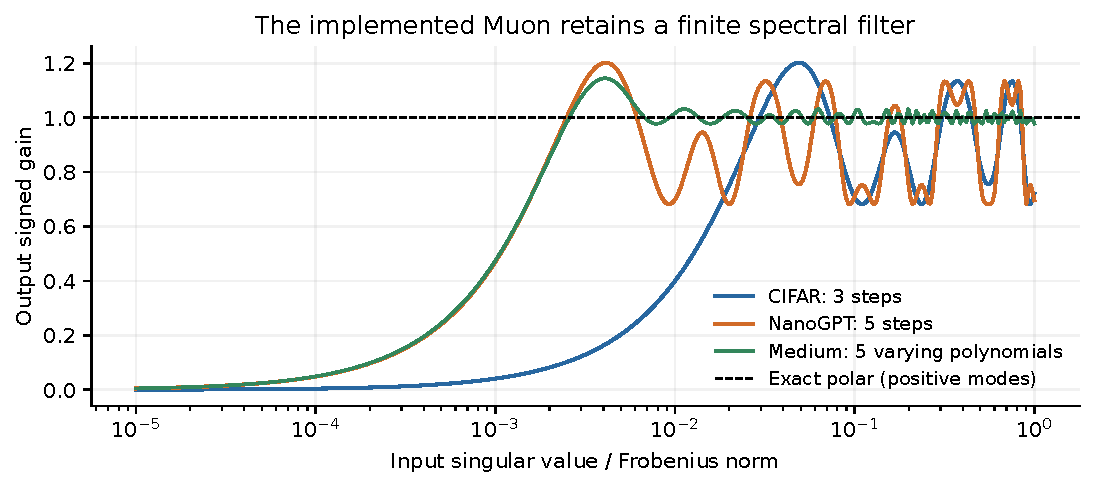
\includegraphics[width=0.90\linewidth]{results/deep_learning/ns_filter.pdf}
\caption{Exact-arithmetic filters from the current scripts. Tiny modes
remain attenuated after a finite number of iterations. This is a property
of the update map, not evidence that attenuated modes are noise.}
\end{figure}

This supplies a useful middle model between hard truncation and an ideal
polar update: preserve every direction with its actual gain $w_i$.
It accommodates every Fanion rank, either with hard indicators or measured
approximate gains, and the extra dense components. Whether weak modes
carry signal or noise must be measured independently.

\subsection{Momentum, dependence, and gradient alignment}

The CIFAR buffer is $B_t=\beta B_{t-1}+g_t$, with $H_t=g_t+\beta B_t$.
The LLM buffer is $M_t=\beta M_{t-1}+(1-\beta)g_t$, with
$H_t=(1-\beta)g_t+\beta M_t$. For \emph{constant} $\beta$ and zero
initialization, $M_t=(1-\beta)B_t$, so the two oracle inputs differ only
by the positive factor $1-\beta$. Ideal homogeneous update maps coincide.
This equivalence need not hold when momentum varies.

For the LLM's deterministic warmup schedule, the normalized input has
weights
\begin{equation}\label{eq:momentum-weights}
 H_t=\sum_{s=0}^t w_{t,s}g_s,\quad
 w_{t,t}=1-\beta_t^2,\quad
 w_{t,s}=\beta_t(1-\beta_s)\prod_{j=s+1}^t\beta_j\ (s<t),\quad
 \sum_s w_{t,s}=1-\beta_t\prod_{j=0}^t\beta_j.
\end{equation}
For constant momentum these reduce to the weights analyzed in
\path{fanion_followup.pdf}. If $g_s=G_s+b_s+\xi_s$, with deterministic
weights and martingale differences $\xi_s$ of second moment at most
$\sigma_s^2$, then
\begin{equation}\label{eq:tracking}
 \E\F{H_t-G_t}\leq
 m_t\E\F{G_t}+\sum_s w_{t,s}\E\F{G_s-G_t}
 +\sum_s w_{t,s}\E\F{b_s}
 +\left(\sum_s w_{t,s}^2\sigma_s^2\right)^{1/2},
 \quad m_t=1-\sum_s w_{t,s}.
\end{equation}
The proof is the triangle inequality and orthogonality of martingale
increments. Changes in parameters \emph{and context rule} enter
$G_s-G_t$. Bias $b_s$ allows reshuffling, document-stream dependence, or
an objective mismatch. This is a conditional noise description, not a
claim that token gradients are IID or that variance divides by token count.

Most importantly, the useful alignment is
$\ip{\nabla F_t}{D_k(H_t)}$, not the always-positive self-alignment
$\ip{H_t}{D_k(H_t)}$. Finite-batch nonlinear transformations may be biased.
\href{https://arxiv.org/abs/2608.04607}{Do, Dereich, and Jentzen (2026)}
give relevant stochastic counterexamples and batch-size-dependent error
analysis for generalized Muon. This does not show failure on these neural
tasks; it rules out treating fixed-batch consistency as automatic.

\section{A finite-horizon theorem for both settings}

Let $x_t$ be the additive LLM state, or the sphere representatives and
auxiliary parameters for the scale-invariant CIFAR idealization. Write the
step as $x_{t+1}=\mathcal R_{x_t}(-\gamma_t V_t)$, using the identity map
for additive updates and a product retraction for CIFAR. In the latter case
the $l$th component of $V_t$ is
$(\eta_{l,t}/\gamma_t)D_{l,t}^{\mathrm{tan}}$ from
\eqref{eq:retraction}. Retain auxiliary updates in the same vector.

\begin{theorem}[Actual-direction descent with objective drift]
Suppose along the executed steps that
\begin{equation}\label{eq:local-upper}
 F_t(\mathcal R_{x_t}(-\gamma_t V_t))
 \leq F_t(x_t)-\gamma_t A_t+\tfrac12\gamma_t^2 B_t,
 \qquad A_t=\ip{\operatorname{grad}F_t(x_t)}{V_t},\quad B_t\geq0.
\end{equation}
Define $\delta_t=F_{t+1}(x_{t+1})-F_t(x_{t+1})$ and assume
$F_T(x_T)\geq F_{\min}$. For every realized trajectory,
\begin{equation}\label{eq:telescope}
 \sum_{t<T}\gamma_t A_t
 \leq F_0(x_0)-F_{\min}
 +\tfrac12\sum_{t<T}\gamma_t^2 B_t
 +\sum_{t<T}\delta_t.
\end{equation}
Replacing the last sum by $\sum_t[\delta_t]_+$ gives a conservative bound.
Taking expectations preserves the inequality when the terms are integrable.
\end{theorem}
\begin{proof}
Add $\delta_t$ to \eqref{eq:local-upper} and sum; the objective values
telescope. No independence or convexity is used. For a fixed context all
$\delta_t$ vanish. An additive upper-model error can be added to the
right-hand side and telescopes in the same way.
\end{proof}

The theorem exposes the quantities a rate comparison must retain:
alignment with the target gradient, curvature of the \emph{actual joint
step}, and context/objective drift. Substituting a global Frobenius
smoothness bound is valid when available but can destroy the comparison.
For example, a structured certificate could bound $B_t$ by
$\chi_t[\sum_l\ip{V_l}{A_lV_lB_l}+C_z(V_z)]$ after proving a
cross-block and nonlinear-residual bound. A raw Hessian-vector product at
one point is an estimate, not itself a certificate over a finite segment.

\paragraph{Optional conditional linear rate.}
In a fixed-objective phase, suppose $A_t>0$, $B_t>0$ and a local
Polyak--\L{}ojasiewicz condition holds above the target loss:
$\F{\operatorname{grad}F}^2\geq2\mu(F-F_*)$.
Define the direction quality $q_t=A_t^2/(B_t\F{\operatorname{grad}F}^2)$
and schedule ratio $\rho_t=\gamma_tB_t/A_t$. If
$\rho_t\in(0,2)$, \eqref{eq:local-upper} gives
\begin{equation}\label{eq:conditional-rate}
 F(x_{t+1})-F_*
 \leq[1-\mu q_t\rho_t(2-\rho_t)](F(x_t)-F_*).
\end{equation}
This follows by writing the decrease as
$A_t^2\rho_t(2-\rho_t)/(2B_t)$. It identifies both a direction factor and
a tuning factor. Neither a global PL condition nor uniformly positive
alignment has been established for these training runs. In a noisy regime
use an expected version with explicit alignment/error assumptions; do not
infer this deterministic rate from same-batch norms.

\section{A more useful hypothesis: comparable Newton corrections}

The key question is which modes need changing in prediction space after
curvature is accounted for. A small gradient singular value can reflect
small curvature, rather than a completed or useless mode. This suggests
testing \emph{broad Newton corrections} instead of assuming a broad raw
gradient spectrum.

At a fixed point let $P_i=u_iv_i^\top$ be the singular directions of the
actual oracle input. For CIFAR replace these by their tangent projections
and use the retraction pullback. Define
\begin{equation}\label{eq:modal-model}
 g_i=\ip{\operatorname{grad}F}{P_i},\qquad
 K_{ij}=\ip{P_i}{\mathcal H P_j},\qquad
 \mathcal Q(d)=\frac{(g^\top d)^2}{d^\top Kd}\quad(g^\top d>0).
\end{equation}
Here $\mathcal H$ is an exact positive quadratic curvature or a valid local
upper model. For an exact quadratic, $\mathcal Q(d)/2$ is the loss decrease
under the best scalar step in direction $\sum_i d_iP_i$.
The rank-$k$ plain direction has $d_i=\boldsymbol1_{i\leq k}$.
Finite Muon uses the gains in \eqref{eq:filter}; F adds $b s_i/\F{H}$
to its spectral weights. For S, retain $\sgn H$ as an extra direction and
extend $g,K$ with its curvature and cross terms. Its component outside the
span of the $P_i$ must not be dropped.

\begin{proposition}[Newton-aligned full polar direction]
Suppose $K\succ0$ on these coordinates and
\begin{equation}\label{eq:newton-alignment}
 g=eK\boldsymbol1,\qquad e>0.
\end{equation}
Then the full ideal Muon direction is the optimal direction in this local
quadratic model, and for every Fanion or hybrid coefficient vector $d$,
\begin{equation}\label{eq:efficiency}
 \frac{\mathcal Q(d)}{\mathcal Q(\boldsymbol1)}
 =\frac{(\boldsymbol1^\top Kd)^2}
 {(\boldsymbol1^\top K\boldsymbol1)(d^\top Kd)}
 =\cos_K^2(\boldsymbol1,d)\leq1.
\end{equation}
Only directions of positive alignment are used. If the actual Newton
correction has zero coordinates outside the polar span, the same statement
holds after adding other directions, including the sign direction.
\end{proposition}
\begin{proof}
The minimizer of the quadratic model has correction
$K^{-1}g=e\boldsymbol1$. Substitution gives \eqref{eq:efficiency}; its
upper bound is Cauchy--Schwarz in the $K$ inner product. The optimal scalar
step for the full polar direction is $e$.
\end{proof}

This is a sufficient, testable structural hypothesis, not a conclusion
deduced from the choice of optimizer. It can also be used with the
\emph{implemented} full-filter direction $w$: the corresponding hypothesis
is $g=eKw$. The local theorem is then exact for that direction. Replacing
an indefinite Hessian by a PSD Gauss--Newton or trust-region upper model
changes the hypothesis and must be stated.

\paragraph{Robustness of the hypothesis.}
If $g=eK\boldsymbol1+h$ and
$\F{K^{-1/2}h}\leq\delta e\F{K^{1/2}\boldsymbol1}$, $0\leq\delta<1$,
then the full polar score relative to the best possible local score obeys
\begin{equation}\label{eq:robust}
 \frac{\mathcal Q(\boldsymbol1)}{g^\top K^{-1}g}
 \geq\left(\frac{1-\delta}{1+\delta}\right)^2.
\end{equation}
Indeed its numerator's alignment is at least
$e(1-\delta)\boldsymbol1^\top K\boldsymbol1$, while
$\F{K^{-1/2}g}\leq e(1+\delta)\F{K^{1/2}\boldsymbol1}$.
Likewise, under exact \eqref{eq:newton-alignment}, a hybrid
$d=a\boldsymbol1+bz$ with
$\F{K^{1/2}bz}\leq\varepsilon a\F{K^{1/2}\boldsymbol1}$,
$a>0$, $\varepsilon<1$, retains at least
$((1-\varepsilon)/(1+\varepsilon))^2$ of the full score. This allows a
negative $b$ as in the manuscript's $\alpha>1$ experiments, provided the
perturbation bound holds; a convex-LMO-sum argument would not cover that case.

\subsection{Every Fanion rank in a solvable curvature model}

Suppose the modal curvature is diagonal with entries $\lambda_i>0$ and
the current modal errors are $e_i>0$. Then $g_i=\lambda_i e_i$.
When $e_i=e$ for all $i$, for the set $I_k$ selected from the oracle input,
\begin{equation}\label{eq:curvature-mass}
 \mathcal Q_k=e^2\sum_{i\in I_k}\lambda_i,\qquad
 \frac{\mathcal Q_r}{\mathcal Q_k}
 =\frac{\sum_{i\leq r}\lambda_i}{\sum_{i\in I_k}\lambda_i}.
\end{equation}
For an exact-gradient input $H=G$, $I_k$ comprises the $k$ largest
$\lambda_i$. For a general momentum input the denominator is at most that
largest-$k$ curvature mass, giving a lower bound on the score ratio.
The effective rank governing the full-versus-top-mode comparison is the
\emph{curvature mass} $\sum_i\lambda_i/\lambda_1$ in the exact-gradient
case, rather than
$(\sum_i\lambda_i)^2/(r\lambda_1^2)$ from a Frobenius surrogate.
For $0<e_{\min}\leq e_i\leq e_{\max}$, even if sorting by gradient and
sorting by curvature differ,
\begin{equation}\label{eq:comparable-errors}
 \frac{\mathcal Q_r}{\mathcal Q_k}
 \geq\left(\frac{e_{\min}}{e_{\max}}\right)^2
 \frac{\sum_i\lambda_i}{\sum_{i\leq k}\lambda_i^{\downarrow}}.
\end{equation}
For the numerator use
$(\sum_i\lambda_i e_i)^2/\sum_i\lambda_i
\geq e_{\min}^2\sum_i\lambda_i$; for the selected denominator use
$\mathcal Q_k\leq e_{\max}^2\sum_{i\in I_k}\lambda_i
\leq e_{\max}^2\sum_{i\leq k}\lambda_i^{\downarrow}$.

For any positive-alignment spectral filter or hybrid weights $d_i$ and
equal errors, the fraction of the optimal decrease is
\begin{equation}\label{eq:cv}
 \frac{\mathcal Q(d)}{e^2\sum_i\lambda_i}
 =\frac{(\E_\pi d)^2}{\E_\pi d^2}
 =\frac{1}{1+\operatorname{Var}_\pi(d)/(\E_\pi d)^2},
 \qquad \pi_i=\frac{\lambda_i}{\sum_j\lambda_j}.
\end{equation}
Thus Muon's near-constant weights can be good in the curvature metric,
F-Muon's weights can be a modest perturbation, and truncated Fanions lose
useful curvature mass. A sign update may have extra off-modal curvature;
its behavior additionally depends on the entry basis. These are explicit
mechanisms for closeness of the full-rank hybrids and weakness of small
ranks, with no universal ordering when the structural hypothesis fails.

\paragraph{An exactly embedded matrix example.}
Take $r=128$, $\lambda_i=i^{-0.9}$, any orthogonal $U,V$, and
\begin{equation}\label{eq:embedded-example}
 f(X)=\tfrac12\ip{X}{AXB},\qquad
 A=U\operatorname{diag}(\sqrt{\lambda_i})U^\top,\quad
 B=V\operatorname{diag}(\sqrt{\lambda_i})V^\top,\quad X_0=UV^\top.
\end{equation}
The gradient is $U\operatorname{diag}(\lambda_i)V^\top$ and
$AP_iB=\lambda_iP_i$, so the example realizes the modal model exactly.
True curvature favors Muon over Neon by $6.82127$, whereas the common
Frobenius surrogate gives ratio $0.363514$ and favors Neon. This shows why
the latter surrogate can give an incorrect ranking without any noise.

For a reproducible random rotation, $a=b=1/2$, and sign scale $0.003$,
the fractions of initial loss removed by the best scalar step are:
\begin{center}
\begin{tabular}{rrrr}
\toprule
Rank & Plain & F & S\\
\midrule
1 & 0.1466 & 0.2594 & 0.2009\\
5 & 0.3562 & 0.3897 & 0.3753\\
128 & 1.0000 & 0.9595 & 0.9961\\
\bottomrule
\end{tabular}
\end{center}
For the three current full-rank polynomial filters the corresponding
fractions are $0.9360$ (CIFAR coefficients, three steps), $0.9714$
(NanoGPT, five steps), and $0.99973$ (Medium's varying polynomials).
These are illustrative exact-arithmetic calculations, not measured network
curvatures, training times, or a fitted explanation of every empirical rank
comparison. Finite-step overshoot, different trajectories, and stochastic
alignment can change the ordering. A local optimum over scalar steps is
also different from the actual fixed schedule.

\begin{figure}[htbp]
\centering
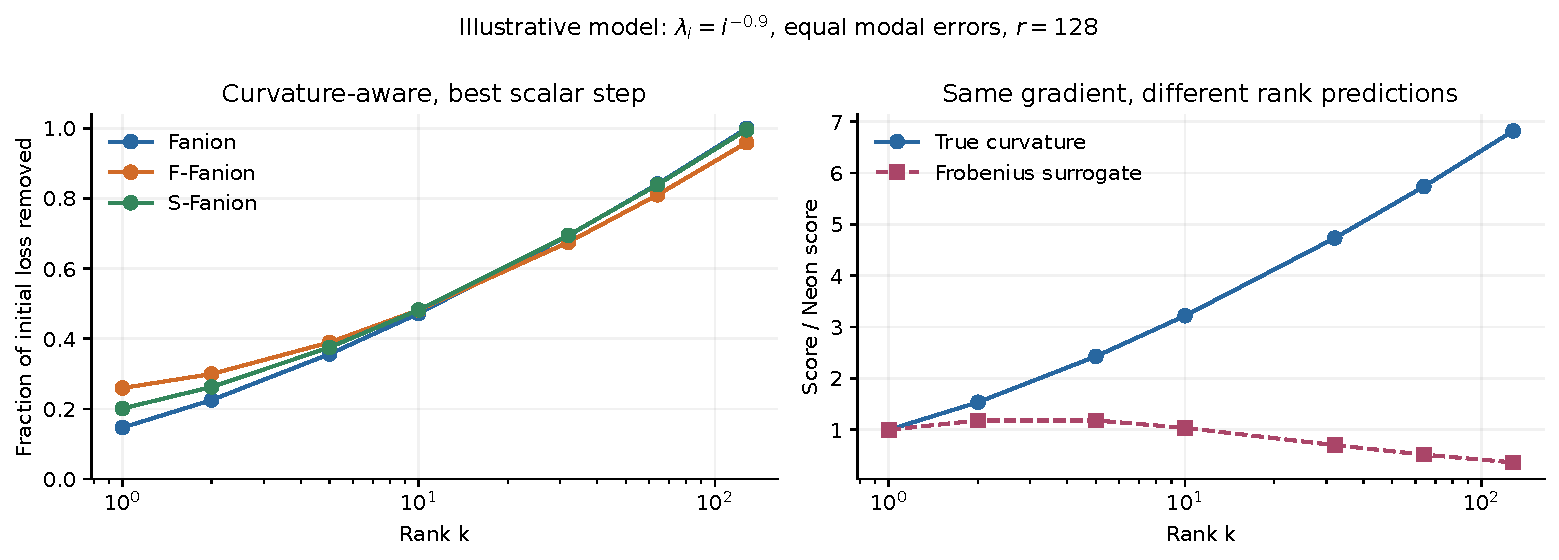
\includegraphics[width=\linewidth]{results/deep_learning/curvature_rank.pdf}
\caption{The same exactly specified matrix model across Fanion ranks.
Left: fraction of loss removed after the best scalar step, including both
hybrids. Right: retaining directional curvature reverses the rank trend
suggested by a Frobenius surrogate. Neither panel uses neural training data.}
\end{figure}

\section{What convergence target matches CIFAR accuracy?}

For $C$ classes and smoothing $\varepsilon\in[0,1)$, let
$q_h=1-\varepsilon+\varepsilon/C$ and $q_l=\varepsilon/C$.
For an example with correct label $y$,
\begin{equation}\label{eq:smoothed-gap}
 \ell_q(p)=H(q)+\KL(q\Vert p),\qquad
 \kappa_{\varepsilon,C}
 =q_h\log\frac{2q_h}{q_h+q_l}
  +q_l\log\frac{2q_l}{q_h+q_l}.
\end{equation}
Use the convention $0\log0=0$.

\begin{proposition}[A sharp mistake cost for smoothed cross-entropy]
If a class other than $y$ has probability at least $p_y$, then
$\ell_q(p)-H(q)\geq\kappa_{\varepsilon,C}$. Consequently, for the
\emph{same} prediction mechanism and distribution,
\begin{equation}\label{eq:error-bound}
 \Pr(\widehat y\ne y)
 \leq\frac{\E\ell_q(p)-H(q)}{\kappa_{\varepsilon,C}}.
\end{equation}
\end{proposition}
\begin{proof}
For a fixed competing class $j$, minimize $\KL(q\Vert p)$ subject to
$p_j\geq p_y$. The optimum pools the two coordinates:
$p_y=p_j=(q_h+q_l)/2$, with $p_i=q_i$ otherwise. This follows from
the Lagrange conditions, or convexity of $-\sum_iq_i\log p_i$.
The resulting KL is \eqref{eq:smoothed-gap}, independent of $j$.
Take the union over possible wrong maximizers pointwise (each has the
same minimum cost), then average the indicator inequality.
\end{proof}

For the actual CIFAR smoothing $\varepsilon=0.2$, $C=10$,
\begin{equation}\label{eq:cifar-constants}
 H(q)=0.86689391,\qquad \kappa_{0.2,10}=0.48773025,
 \qquad \log(q_h/q_l)=\log41=3.71357207.
\end{equation}
Units are natural-log cross-entropy. Perfect training classification does
not require vanishing gradients or attaining $H(q)$: it only requires
the correct class to have the largest probability. Moreover the smoothed
logit optimum has a finite target margin $\log41$; a zero-loss or
unbounded-margin model for unsmoothed separable classification would
misdescribe this experiment.

The inequality links training optimization to training error, or population
loss to population error. For validation accuracy, one additionally needs
the appropriate loss generalization control and a bound on changing the
prediction mechanism (augmentation, frozen BatchNorm statistics, and test
augmentation). A training-mode gradient theorem alone does not rank the
reported validation accuracies. Even \eqref{eq:error-bound} is an upper
bound, so comparing its values cannot prove a strict actual-accuracy ordering.

For LLM evaluation, the target is already held-out mean token cross-entropy.
There is no need to replace it by classification accuracy or by a vanishing
parameter-gradient target. Population versus finite held-out loss still
requires a sampling statement if a statistical claim is intended. The
bounded logit transformation in the NanoGPT script further means that the
usual unrestricted softmax infinite-margin limit is not its literal model.

\section{Measurements that would decide between explanations}

The new structural assumption is not checkable from Frobenius, operator,
and nuclear norms alone. The following measurements at a few shared
checkpoints would make the theory discriminating.
\begin{enumerate}
\item \textbf{Record the actual configuration and displacement.}
For every group save the normalization flag and order, matrix/tensor shape,
learning-rate multipliers, the two hybrid component steps, polynomial
coefficients, momentum convention, and auxiliary update. For CIFAR also
save $W$, $N(W)$, the radial component, and the tangent displacement.
For the LLM save context/window and summed-versus-mean gradient scaling.
\item \textbf{Use an independent probe gradient.}
At the same state and context, form the candidate directions from the
same actual momentum input $H$, then estimate
$\ip{\nabla F_t}{V}$ on fresh training batches/documents. This diagnoses
the update map without its same-batch self-alignment bias. BatchNorm state
must be kept consistent during probes. At each algorithm's own trajectory
also log its own $H$; a common-input counterfactual does not replace that.
\item \textbf{Measure curvature and actual loss change.}
Estimate $V^\top K^{\mathrm{GN}}V$ by a joint Jacobian-vector product and
compare with a Hessian-vector product or symmetric small loss probes.
Include matrix/auxiliary and cross-layer interactions, and for CIFAR
probe the actual retraction. Check finite-step Taylor error rather than
treating a pointwise curvature as an upper bound. Both
$A^2/B$ and the actual scheduled decrease $\gamma A-\gamma^2B/2$ matter.
\item \textbf{Resolve all ranks.}
Log leading singular values of $H$ beyond ranks 1 and 5, the polynomial
gains, and $g_i=\ip{G_{\mathrm{probe}}}{P_i}$. Estimate the modal Gram matrix
or selected diagonal/cross terms. The question is whether the inferred
correction $K^{-1}g$ is broad and approximately constant in the polar
modes, and whether curvature mass outside the first $k$ directions is
large. Do not infer this from a heavy-tailed gradient spectrum alone.
\item \textbf{Separate tuning and generalization.}
Compare inherited, independently tuned, and tangent/Frobenius-matched
rank schedules. Keep normalized and unnormalized CIFAR runs separate.
For an accuracy explanation, examine train loss, validation loss, and the
normalization/evaluation gap alongside accuracy. For LLMs compare fixed
context phases or report the context drift.
\end{enumerate}

These measurements yield competing predictions. If the useful correction
is broad but gradients are anisotropic, the curvature model predicts a
Muon advantage and near-equivalence of small full-rank perturbations.
If weak modes are mostly noise, their independent alignments will be small
or negative and a truncated/soft-filter method can be better. If the gap
largely vanishes after rank-dependent retuning, step scale explained much
of the original inherited-hyperparameter gap. The results should be used
to select a structural hypothesis, not to assert that one already holds.

\section{What is established, and what is still a hypothesis}

Established here are the exact normalization reindexing, finite-filter
representation, variable-momentum weights, drift-aware descent theorem,
local curvature/Newton comparison for every rank, the smoothed-loss
classification bound, and an exactly embedded example reversing a
Frobenius-based rank prediction. The analysis script passes 3,378 numerical
checks and records input hashes and limitations in
\path{results/deep_learning/summary.json}. Its examples are deterministic
mathematical diagnostics, with random seed 20261021, not neural experiments.

For the article, the strongest defensible description is:
\emph{``Muon can exploit a broad useful correction in the network's local
curvature geometry. Low-rank Fanions can miss a substantial fraction of
that correction; full-rank F and S perturbations can retain most of it.
The explanation depends on projected/functional alignment, directional
curvature, and the effective schedule, which are not fixed by asymptotic
exponents or by three raw gradient norms.''}
This remains a proposed mechanism for the CIFAR/LLM results until the
stated quantities are measured. It does not establish a universal optimizer
ordering, a global neural convergence rate, or a generalization theorem.

\paragraph{Reproduce.}
From the repository root:
\begin{verbatim}
python theory_attempts/deep_learning_analysis.py
python theory_attempts/build_report.py --stem deep_learning_model
\end{verbatim}
The CSV files contain the full rank curves, nominal CIFAR scales, and
spectral filters; standalone figures are provided as PDF and PNG.
\path{paper_insert_deep_learning.tex} is a compact candidate discussion
and proposition for the submission, which remains unmodified.

\section*{References and relation to existing work}
\begin{enumerate}
\item Martens and Grosse (2015),
\href{https://proceedings.mlr.press/v37/martens15.html}{Optimizing Neural
Networks with Kronecker-factored Approximate Curvature}.
Provides the established Fisher-block/Kronecker motivation. We use this
as a possible model, not as a theorem certifying the full neural Hessian.
\item van Laarhoven (2017),
\href{https://arxiv.org/abs/1706.05350}{L2 Regularization versus Batch and
Weight Normalization}. Studies scale invariance and effective learning
rates under normalization. The normalization-before-step identity here
is a direct calculation for this repository's order of operations.
\item Jordan (2024),
\href{https://kellerjordan.github.io/posts/muon/}{Muon: An optimizer for
hidden layers in neural networks}. Describes polynomial action on singular
values, mixed parameter groups, and the motivation for amplifying weaker
directions. Our mode model gives a conditional curvature interpretation;
it is not a claim that the spectral-filter representation is new.
\item Do, Dereich, and Jentzen (2026),
\href{https://arxiv.org/abs/2608.04607}{On MUON optimization: From
non-convergence to an error analysis with Polar Express and the
Newton--Schulz polynomial from implementations}. Gives generalized
polynomial-Muon analysis and stochastic examples with a batch-size error
term, reinforcing the need to retain noise-induced alignment error.
\item For prior structured convergence results and multiblock norm models,
see \href{https://arxiv.org/abs/2511.11466}{Kovalev and Borodich (v2, 2026)},
\href{https://arxiv.org/abs/2505.23737}{Shen et al. (v3, 2026)},
and \href{https://arxiv.org/abs/2510.09827}{Crawshaw et al. (2025)}.
These were discussed in the earlier attempts. The present note contributes
an experiment-specific description and conditional mechanisms, not a
priority or novelty claim for standard local descent and metric-angle facts.
\end{enumerate}
\end{document}
